\documentclass{article}

% if you need to pass options to natbib, use, e.g.:
% \PassOptionsToPackage{numbers, compress}{natbib}
% before loading nips_2017
%
% to avoid loading the natbib package, add option nonatbib:
% \usepackage[nonatbib]{nips_2017}

\usepackage{nips_2017}
\usepackage{dsfont}
% to compile a camera-ready version, add the [final] option, e.g.:
% \usepackage[final]{nips_2017}

\usepackage[utf8]{inputenc} % allow utf-8 input
\usepackage[T1]{fontenc}    % use 8-bit T1 fonts
\usepackage{hyperref}       % hyperlinks
\usepackage{url}            % simple URL typesetting
\usepackage{booktabs}       % professional-quality tables
\usepackage{amsfonts}       % blackboard math symbols
\usepackage{nicefrac}       % compact symbols for 1/2, etc.
\usepackage{microtype}      % microtypography

\usepackage{graphicx} % more modern
%\usepackage{epsfig} % less modern
\usepackage{subfig} 
\usepackage{fancyvrb}

\usepackage{caption}
\usepackage{subcaption}

\fvset{fontsize=\footnotesize}


\usepackage{multirow}
\usepackage{array}

\usepackage{amssymb}
\usepackage{listings}
\usepackage{wrapfig}
\usepackage{tabularx}


\usepackage{verbatim}
 \usepackage{booktabs}
 % For algorithms
\usepackage{algorithm}
\usepackage{algorithmic}
\usepackage{tikz}
\usetikzlibrary{fit}
% As of 2011, we use the hyperref package to produce hyperlinks in the
% resulting PDF.  If this breaks your system, please commend out the
% following usepackage line and replace \usepackage{icml2016} with
% \usepackage[nohyperref]{icml2016} above.
\usepackage{amsmath}
\usepackage{hyperref}
\DeclareMathOperator*{\argmin}{arg\,min} % thin space, limits underneath in displays
\DeclareMathOperator{\argmin}{argmin} % no space, limits underneath in displays

\newcommand{\expect}{\mathds{E}} %{{\rm I\kern-.3em E}}
\newcommand{\probability}{\mathds{P}} %{{\rm I\kern-.3em P}}


\title{Inferring Graphics Programs from Images}

% The \author macro works with any number of authors. There are two
% commands used to separate the names and addresses of multiple
% authors: \And and \AND.
%
% Using \And between authors leaves it to LaTeX to determine where to
% break the lines. Using \AND forces a line break at that point. So,
% if LaTeX puts 3 of 4 authors names on the first line, and the last
% on the second line, try using \AND instead of \And before the third
% author name.

\author{
  David S.~Hippocampus\thanks{Use footnote for providing further
    information about author (webpage, alternative
    address)---\emph{not} for acknowledging funding agencies.} \\
  Department of Computer Science\\
  Cranberry-Lemon University\\
  Pittsburgh, PA 15213 \\
  \texttt{hippo@cs.cranberry-lemon.edu} \\
  %% examples of more authors
  %% \And
  %% Coauthor \\
  %% Affiliation \\
  %% Address \\
  %% \texttt{email} \\
  %% \AND
  %% Coauthor \\
  %% Affiliation \\
  %% Address \\
  %% \texttt{email} \\
  %% \And
  %% Coauthor \\
  %% Affiliation \\
  %% Address \\
  %% \texttt{email} \\
  %% \And
  %% Coauthor \\
  %% Affiliation \\
  %% Address \\
  %% \texttt{email} \\
}

\begin{document}
% \nipsfinalcopy is no longer used

\maketitle

\begin{abstract}
\end{abstract}

\section{Introducing visual programs}

\textbf{Comment for reader: this paragraph is a little grandiose and goes
  beyond what we've actually done. But these are the kinds of things
  that motivate the work, and I think that in some form these ideas
  should be in the introduction or the conclusion.} How could an agent go from noisy,
high-dimensional perceptual input to a symbolic, abstract object, like
a computer program?  Here we consider this problem within the context
of \emph{graphics program synthesis}.  We develop an approach for
converting natural images, such as hand drawings, into executable
source code for drawing the original image.
The source code captures not just the objects in the image,
but also describes their geometric relationships.

High dimensional perceptual input is ill matched to the abstract
semantics of a programming language. But programs with constructs like
recursion or iteration produce a simpler \emph{execution trace} of
primitive actions. Our hypothesis is that the execution trace of the
program is better aligned with the perceptual input, and that the
trace can act as a kind of bridge between perception and programs. We
test this hypothesis by developing a model that learns to map from an
image to the execution trace of the graphics program that drew it.
With the execution trace in hand, we can bring to bear techniques from
the program synthesis community to recover the latent graphics program.



In this work we consider programs that draw diagrams, similar to those found in papers.

We develop a hybrid architecture for inferring graphics programs.  Our
approach uses a deep network infer an execution trace from an image;
this recovers primitive drawing operations like lines, circles, or
arrows.  For added robustness we use the deep network as a proposal
distribution for a stochastic search over execution traces.
Finally we use techniques in the program synthesis community to
recover the program from its trace.

Each of these three components -- the deep network, the stochastic
search, the program synthesizer -- confers its own advantages. From
the deep network we get a very fast system that can recover plausible
execution traces in about a minute. From the stochastic search we get
added robustness; essentially the stochastic search can correct
mistakes made by the deep network's proposals.  From the program
synthesizer we get abstraction: our system recovers coordinate
transformations, for loops, and subroutines, which are useful for
downstream tasks.

\section{Neural architecture for inferring image parses}

We developed a deep network architecture for efficiently inferring a
execution trace, $T$, from an image, $I$.  Our model constructs the
trace one drawing command at a time.  When predicting the next drawing
command, the network takes as input the target image $I$ as well as
the rendered output of previous drawing commands.  Intuitively, the
network looks at the image it wants to explain, as well as what it has
already drawn.  It then decides either to stop drawing or proposes
another drawing command to add to the execution trace; if it decides
to continue drawing, the predicted primitive is rendered to its
``canvas'' and the process repeats.

Figure~\ref{architecture} illustrates this architecture.  We first
pass the target image and a rendering of the trace so far to a
convolutional network. Given the features extracted by the
convolutionional network, a multilayer perceptron then predicts a
distribution over the next drawing command to add to the trace.  We
predict the drawing command token-by-token, and condition each token
both on the image features and on the previously generated tokens.
For example, the network first decides to emit the \verb|CIRCLE| token
conditioned on the image features, then it emits the $x$ coordinate of
the circle conditioned on the image features and the \verb|CIRCLE|
token, and finally it predicts the $y$ coordinate of the circle
conditioned on the image features, the \verb|CIRCLE| token, and the
$x$ coordinate.

The distribution over the next drawing command factorizes:
\begin{equation}
  \probability_\theta [t_1t_2\cdots t_K | I,T] = \prod_{k = 1}^K \probability_\theta [t_k | f_\theta(I,\text{render}(T)), \{t_j\}_{j = 1}^{k - 1}]
\end{equation}
where $t_1t_2\cdots t_K$ are the tokens in the drawing command, $I$ is
the target image, $T$ is an execution trace, $\theta$ are the
parameters of the neural network, and $f_\theta(\cdot,\cdot)$ is the
image feature extractor (convolutional network). The distribution over
execution traces factorizes as:
\begin{equation}
  \probability_\theta [T|I] = \prod_{n = 1}^{|T|} \probability_\theta [T_n | I,T_{1:(n-1)}]\times\probability_\theta [\verb|STOP| | I,T]\label{objective}
\end{equation}
where $|T|$ is the length of execution trace $T$, and the \verb|STOP|
token is emitted by the network to signal that the execution trace
explains the image.

We train the network by sampling execution traces $T$ and target
images $I$ for randomly generated scenes, and maximizing
(\ref{objective}) wrt $\theta$ by gradient ascent. Despite the
architecture being recurrent, training is fully supervised. In a
sense, this model is like an autoregressive variant of AIR.

%% When we
%% have the generative model (the rendering function) and treat the trace
%% as fully observed, we need not solve an unsupervised or reinforcement
%% learning problem.

\begin{figure}
  \begin{tikzpicture}
  \node[draw,ultra thick,anchor = west,inner sep=0pt,label=below:Target image: $I$](observation) at (0,0) {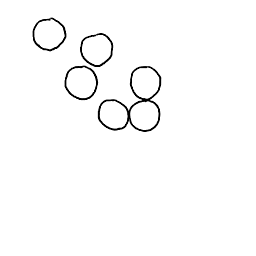
\includegraphics[width = 3cm]{figures/expert-18.png}};
  \node[draw,thick,anchor = west,inner sep=0pt,minimum width = 3cm,minimum height = 3cm,label=below:Canvas: render$(T)$] (canvas) at (0,-5) {};
  % draw partial image on canvas
  \draw (0.5cm,-4cm) circle (0.1875cm);
  \draw (1.2cm,-4.3) circle (0.1875cm);
  \draw (0.85cm,-4.6) circle (0.1875cm);

  \node[draw,thick,anchor = west,inner sep=0pt,minimum width = 3cm,minimum height = 3cm] (CNN) at (4.5,-2.5) {CNN};

  \node[rotate = -90,draw,thick,inner sep=0pt,minimum width = 3cm,minimum height = 0.5cm] (features) at ([xshift = 1cm]CNN.east) {Image features};

  \node[draw,thick,circle,minimum size = 1cm](c1) at ([xshift = 1.5cm]features.north);
  \node(l1) at ([yshift = -2cm]c1.south) {\verb|CIRCLE(|};
  \node[draw,thick,circle,minimum size = 1cm](c2) at ([xshift = 1cm]c1.east);
  \draw[->,thick] (c1.south) -- (l1.north);
  \node(l2) at ([yshift = -2cm]c2.south) {\verb|X=3,|};
  \draw[->,thick] (c2.south) -- (l2.north);
  \node[draw,thick,circle,minimum size = 1cm](c3) at ([xshift = 1cm]c2.east);
  \node(l3) at ([yshift = -2cm]c3.south) {\verb|Y=14)|};
  \draw[->,thick] (c3.south) -- (l3.north);

  
  \draw[->,thick] (features.north) -- (c1.west);
  \draw[->,thick] (c1.east) -- (c2.west);
  \draw[->,thick] (c2.east) -- (c3.west);

  \node(next)[draw,fit = (l1) (l2) (l3), dashed, label = below:{Next line of code}] {};

  \draw[->,thick,dashed] (next.west) -- node[below] {Renderer: \LaTeX} (canvas.east);
  
  \draw[->,thick] (canvas.east) -- ([yshift = -0.5cm]CNN.west);
  \draw[->,thick] (observation.east) -- ([yshift = 0.5cm]CNN.west);
  \draw[->,thick] (CNN.east) -- (features.south);
%  \draw[]
  
%  \node at (canvas.x,canvas.y) {Canvas};
\end{tikzpicture}
\caption{Our neural architecture for inferring the execution trace of a graphics program from its output.}  \label{architecture}
  \end{figure}

\begin{table}
\begin{tabular}{ll}\toprule
  \begin{tabular}{l}
    \verb|CIRCLE|$(x,y)$
    \end{tabular}& Circle at $(x,y)$\\
  \begin{tabular}{l}
    \verb|RECTANGLE|$(x_1,y_1,x_2,y_2)$
    \end{tabular}&Rectangle with corners at $(x_1,y_1)$ \& $(x_2,y_2)$\\
  \begin{tabular}{l}
    \verb|LINE|$(x_1,y_1,x_2,y_2,$\\
    \hspace{1cm}$\text{arrow}\in\{0,1\},\text{dashed}\in\{0,1\})$
    \end{tabular}&Line from $(x_1,y_1)$ to  $(x_2,y_2)$, optionally with an arrow and/or dashed\\
  \begin{tabular}{l}
    \verb|STOP|
  \end{tabular}&Finishes execution trace inference
\\  \bottomrule
\end{tabular}
\caption{The deep network in (\ref{architecture}) predicts drawing commands, shown above.}
\label{drawingCommandTable}
\end{table}

\section{Generalizing to hand drawings}

\begin{figure}
  \begin{minipage}[b]{0.3\textwidth}
    \centering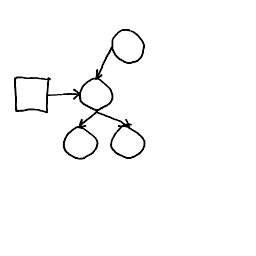
\includegraphics[width = 3cm]{figures/expert-60.png}
    \subcaption{(a)}
  \end{minipage}%
  \begin{minipage}[t]{0.3\textwidth}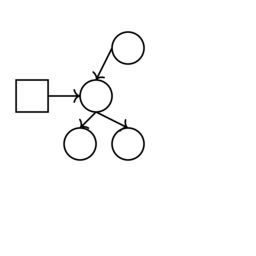
\includegraphics[width = 3cm]{figures/60-groundTruth.png}
    \subcaption{(b)}
  \end{minipage}\\
  \begin{minipage}[t]{0.3\textwidth}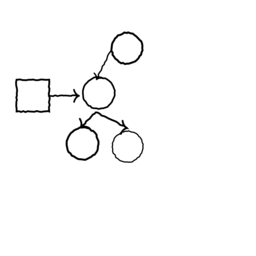
\includegraphics[width = 3cm]{figures/60-1.png}
    \subcaption{(c)}
  \end{minipage}%
  \begin{minipage}[t]{0.3\textwidth}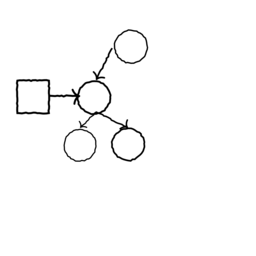
\includegraphics[width = 3cm]{figures/60-2.png}
    \subcaption{(d)}
  \end{minipage}
  \caption{(a): a hand drawing. (b): Rendering of the parse our model infers for (a). We can generalize to hand drawings like these because we train the model on images corrupted by a noise process designed to resemble the kind of noise introduced by hand drawings - see (c) \& (d) for noisy renderings of (b).}
  \end{figure}

\section{Synthesizing graphics programs from execution traces}

\begin{table}
  \begin{tabular}{rl}
  Program$\to$&Command; $\cdots$; Command\\
  Command$\to$&\texttt{CIRCLE}(Expression,Expression)\\
  Command$\to$&\texttt{RECTANGLE}(Expression,Expression,Expression,Expression)\\
  Command$\to$&\texttt{LINE}(Expression,Expression,Expression,Expression,Boolean,Boolean)\\
  Command$\to$&\texttt{FOR}$(0\leq \text{Var}  < \text{Expression})$\texttt{ \{ }Program\texttt{ \}}\\
  Command$\to$&\texttt{REFLECT}$(\text{Axis})$\texttt{ \{ }Program\texttt{ \}}\\
  Expression$\to$&\mathcal{Z}\texttt{ * }Var\texttt{ + }\mathcal{Z}\\
  Var$\to$&A free (unused) variable\\
  \mathcal{Z}$\to$&an integer\\
  Axis$\to$&\texttt{X = }\mathcal{Z}\\
  Axis$\to$&\texttt{Y = }\mathcal{Z}
  \end{tabular}
  \caption{Grammar over graphics programs. We allow loops (\texttt{FOR}), vertical/horizontal reflections (\texttt{REFLECT}), and affine transformations (\mathcal{Z}\texttt{ * }Var\texttt{ + }\mathcal{Z}).}
  \end{table}

\section{Neural networks for guiding SMC}



Let $L(\cdot | \cdot):\text{image}^2\to \mathcal{R}$ be our likelihood
function: it takes two images, an observed target image and a
hypothesized program output, and gives the likelihood of the observed
image conditioned on the program output. We want to sample from:
\begin{equation}
\probability [p|x]  \propto L(x | \text{render}(p)) \probability [p]
\end{equation}
where $\probability [p]$ is the prior probability of program $p$, and $x$ is the observed image.

Let $p$ be a program with $L$ lines, which we will write as $p = (p_1,p_2,\cdots,p_L)$. Assume the prior factors into:
\begin{equation}
  \probability [p]\propto \prod_{l\leq L}\probability [p_l]
\end{equation}
Define the distribution $q_L(\cdot)$, which happens to be proportional to the above posterior:
\begin{equation}
  q_L(p_1,p_2,\cdots,p_{L - 1},p_L)\propto q_{L - 1}(p_1,p_2,\cdots,p_{L - 1})\times \frac{L(x | \text{render}(p_1,p_2,\cdots,p_{L - 1},p_L))}{L(x | \text{render}(p_1,p_2,\cdots,p_{L - 1}))}\times\probability [p_L]
\end{equation}
Now suppose we have some samples from $q_{L - 1}(\cdot)$, and that we
then sample a $p_L$ from a distribution proportional to $\frac{L(x |
  \text{render}(p_1,p_2,\cdots,p_{L - 1},p_L))}{L(x |
  \text{render}(p_1,p_2,\cdots,p_{L - 1}))}\times\probability [p_L]$.
The resulting programs $p$ are distributed according to $q_L$, and so
are also distributed according to $\probability [p|x]$.

How do we sample $p_L$ from a distribution proportional to $\frac{L(x
  | \text{render}(p_1,p_2,\cdots,p_{L - 1},p_L))}{L(x |
  \text{render}(p_1,p_2,\cdots,p_{L - 1}))}\times\probability [p_L]$?
We have a neural network that takes as input the target image $x$ and
the program so far, and produces a distribution over next lines of
code ($p_L$).  We write $\text{NN}(p_L | p_1,\cdots,p_{L - 1};x)$ for
the distribution output by the neural network. So we can sample from NN and then weight the samples by:
\begin{equation}
  w(p_L) = \frac{\probability [p_L]}{\text{NN}(p_L | p_1,\cdots,p_{L - 1};x)}\times \frac{L(x | \text{render}(p_1,p_2,\cdots,p_{L - 1},p_L))}{L(x | \text{render}(p_1,p_2,\cdots,p_{L - 1}))}
\end{equation}
Then we can resample from these now weighted samples to get a new
population of particles (here programs are particles), where each
program now has $L$ lines instead of $L - 1$.

This procedure can be seen as a particle filter, where each successive
latent variable is another line of code, and the emission
probabilities are successive ratios of likelihoods under $L(\cdot |
\cdot)$.

\textbf{Comments for Dan}. Right now I'm not actually sampling from
the neural network - instead, I enumerate the top few hundred lines of
code suggested by the network, and then weight them by their
likelihoods.
So actually the form of NN is:
\begin{equation}
  \text{NN}(p_L | p_1,\cdots,p_{L - 1};x)\propto \begin{cases}
    1,&\text{ if }p_L \in \text{top hundred neural network proposals}\\
0,&\text{otherwise}.    \end{cases}
\end{equation}
Do you think this is a problem? The neural network puts almost all of its mass on a few guesses.
In order to get the correct line of code I sometimes need to get something like the 50th  top guess,
so I don't want to literally just sample from the distribution suggested by the neural network.


  \begin{algorithm}[tb]
   \caption{Neurally guided SMC}
   \label{guideAlgorithm}
\begin{algorithmic}
  \STATE {\bfseries Input:} Neural network NN, beam size $N$, maximum length $L$, target image $x$
  \STATE {\bfseries Output:} Samples of the program trace
  \STATE Set $B_0 = \{\text{empty program}\}$
  \FOR{$1\leq l\leq L$}
  \FOR{$1\leq n\leq N$}
  \STATE{ $p_n\sim \text{Uniform}(B_{l - 1})$}
  \STATE{ $p'_{n}\sim \text{NN}(\text{render}(p),x)$}
  \STATE{ Define $r_n = p'_n\cdot p_n$}
  \STATE{ Set $\tilde{w}(r_n) = \frac{L(x|r_n)}{L(x|p_n)}\times\frac{\probability [p'_n]}{\probability [p'_n = \text{NN}(\text{render}(p),x)]}$}
  \ENDFOR
  \STATE{ Define $w(p) = \frac{\tilde{w}(p)}{\sum_{p'}\tilde{w}(p')}$}
  \STATE{ Set $B_l$ to be $N$ samples from $r_n$ distributed according to $w(\cdot)$}
  \ENDFOR
  \STATE {\bfseries return} $\{p : p\in B_{l\leq L}, p \text{ is finished}\}$
\end{algorithmic}
  \end{algorithm}


\section{Submission of papers to NIPS 2017}

NIPS requires electronic submissions.  The electronic submission site
is
\begin{center}
  \url{https://cmt.research.microsoft.com/NIPS2017/}
\end{center}

Please read carefully the instructions below and follow them
faithfully.

\subsection{Style}

Papers to be submitted to NIPS 2017 must be prepared according to the
instructions presented here. Papers may only be up to eight pages
long, including figures. This does not include acknowledgments and 
cited references which are allowed on subsequent pages.
Papers that exceed these limits will not be reviewed, or in any
other way considered for presentation at the conference.

The margins in 2017 are the same as since 2007, which allow for
$\sim$$15\%$ more words in the paper compared to earlier years.

Authors are required to use the NIPS \LaTeX{} style files obtainable
at the NIPS website as indicated below. Please make sure you use the
current files and not previous versions. Tweaking the style files may
be grounds for rejection.

\subsection{Retrieval of style files}

The style files for NIPS and other conference information are
available on the World Wide Web at
\begin{center}
  \url{http://www.nips.cc/}
\end{center}
The file \verb+nips_2017.pdf+ contains these instructions and
illustrates the various formatting requirements your NIPS paper must
satisfy.

The only supported style file for NIPS 2017 is \verb+nips_2017.sty+,
rewritten for \LaTeXe{}.  \textbf{Previous style files for \LaTeX{}
  2.09, Microsoft Word, and RTF are no longer supported!}

The new \LaTeX{} style file contains two optional arguments:
\verb+final+, which creates a camera-ready copy, and \verb+nonatbib+,
which will not load the \verb+natbib+ package for you in case of
package clash.

At submission time, please omit the \verb+final+ option. This will
anonymize your submission and add line numbers to aid review.  Please
do \emph{not} refer to these line numbers in your paper as they will
be removed during generation of camera-ready copies.

The file \verb+nips_2017.tex+ may be used as a ``shell'' for writing
your paper. All you have to do is replace the author, title, abstract,
and text of the paper with your own.

The formatting instructions contained in these style files are
summarized in Sections \ref{gen_inst}, \ref{headings}, and
\ref{others} below.

\section{General formatting instructions}
\label{gen_inst}

The text must be confined within a rectangle 5.5~inches (33~picas)
wide and 9~inches (54~picas) long. The left margin is 1.5~inch
(9~picas).  Use 10~point type with a vertical spacing (leading) of
11~points.  Times New Roman is the preferred typeface throughout, and
will be selected for you by default.  Paragraphs are separated by
\nicefrac{1}{2}~line space (5.5 points), with no indentation.

The paper title should be 17~point, initial caps/lower case, bold,
centered between two horizontal rules. The top rule should be 4~points
thick and the bottom rule should be 1~point thick. Allow
\nicefrac{1}{4}~inch space above and below the title to rules. All
pages should start at 1~inch (6~picas) from the top of the page.

For the final version, authors' names are set in boldface, and each
name is centered above the corresponding address. The lead author's
name is to be listed first (left-most), and the co-authors' names (if
different address) are set to follow. If there is only one co-author,
list both author and co-author side by side.

Please pay special attention to the instructions in Section \ref{others}
regarding figures, tables, acknowledgments, and references.

\section{Headings: first level}
\label{headings}

All headings should be lower case (except for first word and proper
nouns), flush left, and bold.

First-level headings should be in 12-point type.

\subsection{Headings: second level}

Second-level headings should be in 10-point type.

\subsubsection{Headings: third level}

Third-level headings should be in 10-point type.

\paragraph{Paragraphs}

There is also a \verb+\paragraph+ command available, which sets the
heading in bold, flush left, and inline with the text, with the
heading followed by 1\,em of space.

\section{Citations, figures, tables, references}
\label{others}

These instructions apply to everyone.

\subsection{Citations within the text}

The \verb+natbib+ package will be loaded for you by default.
Citations may be author/year or numeric, as long as you maintain
internal consistency.  As to the format of the references themselves,
any style is acceptable as long as it is used consistently.

The documentation for \verb+natbib+ may be found at
\begin{center}
  \url{http://mirrors.ctan.org/macros/latex/contrib/natbib/natnotes.pdf}
\end{center}
Of note is the command \verb+\citet+, which produces citations
appropriate for use in inline text.  For example,
\begin{verbatim}
   \citet{hasselmo} investigated\dots
\end{verbatim}
produces
\begin{quote}
  Hasselmo, et al.\ (1995) investigated\dots
\end{quote}

If you wish to load the \verb+natbib+ package with options, you may
add the following before loading the \verb+nips_2017+ package:
\begin{verbatim}
   \PassOptionsToPackage{options}{natbib}
\end{verbatim}

If \verb+natbib+ clashes with another package you load, you can add
the optional argument \verb+nonatbib+ when loading the style file:
\begin{verbatim}
   \usepackage[nonatbib]{nips_2017}
\end{verbatim}

As submission is double blind, refer to your own published work in the
third person. That is, use ``In the previous work of Jones et
al.\ [4],'' not ``In our previous work [4].'' If you cite your other
papers that are not widely available (e.g., a journal paper under
review), use anonymous author names in the citation, e.g., an author
of the form ``A.\ Anonymous.''

\subsection{Footnotes}

Footnotes should be used sparingly.  If you do require a footnote,
indicate footnotes with a number\footnote{Sample of the first
  footnote.} in the text. Place the footnotes at the bottom of the
page on which they appear.  Precede the footnote with a horizontal
rule of 2~inches (12~picas).

Note that footnotes are properly typeset \emph{after} punctuation
marks.\footnote{As in this example.}

\subsection{Figures}

All artwork must be neat, clean, and legible. Lines should be dark
enough for purposes of reproduction. The figure number and caption
always appear after the figure. Place one line space before the figure
caption and one line space after the figure. The figure caption should
be lower case (except for first word and proper nouns); figures are
numbered consecutively.

You may use color figures.  However, it is best for the figure
captions and the paper body to be legible if the paper is printed in
either black/white or in color.
\begin{figure}[h]
  \centering
  \fbox{\rule[-.5cm]{0cm}{4cm} \rule[-.5cm]{4cm}{0cm}}
  \caption{Sample figure caption.}
\end{figure}

\subsection{Tables}

All tables must be centered, neat, clean and legible.  The table
number and title always appear before the table.  See
Table~\ref{sample-table}.

Place one line space before the table title, one line space after the
table title, and one line space after the table. The table title must
be lower case (except for first word and proper nouns); tables are
numbered consecutively.

Note that publication-quality tables \emph{do not contain vertical
  rules.} We strongly suggest the use of the \verb+booktabs+ package,
which allows for typesetting high-quality, professional tables:
\begin{center}
  \url{https://www.ctan.org/pkg/booktabs}
\end{center}
This package was used to typeset Table~\ref{sample-table}.

\begin{table}[t]
  \caption{Sample table title}
  \label{sample-table}
  \centering
  \begin{tabular}{lll}
    \toprule
    \multicolumn{2}{c}{Part}                   \\
    \cmidrule{1-2}
    Name     & Description     & Size ($\mu$m) \\
    \midrule
    Dendrite & Input terminal  & $\sim$100     \\
    Axon     & Output terminal & $\sim$10      \\
    Soma     & Cell body       & up to $10^6$  \\
    \bottomrule
  \end{tabular}
\end{table}

\section{Final instructions}

Do not change any aspects of the formatting parameters in the style
files.  In particular, do not modify the width or length of the
rectangle the text should fit into, and do not change font sizes
(except perhaps in the \textbf{References} section; see below). Please
note that pages should be numbered.

\section{Preparing PDF files}

Please prepare submission files with paper size ``US Letter,'' and
not, for example, ``A4.''

Fonts were the main cause of problems in the past years. Your PDF file
must only contain Type 1 or Embedded TrueType fonts. Here are a few
instructions to achieve this.

\begin{itemize}

\item You should directly generate PDF files using \verb+pdflatex+.

\item You can check which fonts a PDF files uses.  In Acrobat Reader,
  select the menu Files$>$Document Properties$>$Fonts and select Show
  All Fonts. You can also use the program \verb+pdffonts+ which comes
  with \verb+xpdf+ and is available out-of-the-box on most Linux
  machines.

\item The IEEE has recommendations for generating PDF files whose
  fonts are also acceptable for NIPS. Please see
  \url{http://www.emfield.org/icuwb2010/downloads/IEEE-PDF-SpecV32.pdf}

\item \verb+xfig+ "patterned" shapes are implemented with bitmap
  fonts.  Use "solid" shapes instead.

\item The \verb+\bbold+ package almost always uses bitmap fonts.  You
  should use the equivalent AMS Fonts:
\begin{verbatim}
   \usepackage{amsfonts}
\end{verbatim}
followed by, e.g., \verb+\mathbb{R}+, \verb+\mathbb{N}+, or
\verb+\mathbb{C}+ for $\mathbb{R}$, $\mathbb{N}$ or $\mathbb{C}$.  You
can also use the following workaround for reals, natural and complex:
\begin{verbatim}
   \newcommand{\RR}{I\!\!R} %real numbers
   \newcommand{\Nat}{I\!\!N} %natural numbers
   \newcommand{\CC}{I\!\!\!\!C} %complex numbers
\end{verbatim}
Note that \verb+amsfonts+ is automatically loaded by the
\verb+amssymb+ package.

\end{itemize}

If your file contains type 3 fonts or non embedded TrueType fonts, we
will ask you to fix it.

\subsection{Margins in \LaTeX{}}

Most of the margin problems come from figures positioned by hand using
\verb+\special+ or other commands. We suggest using the command
\verb+\includegraphics+ from the \verb+graphicx+ package. Always
specify the figure width as a multiple of the line width as in the
example below:
\begin{verbatim}
   \usepackage[pdftex]{graphicx} ...
   \includegraphics[width=0.8\linewidth]{myfile.pdf}
\end{verbatim}
See Section 4.4 in the graphics bundle documentation
(\url{http://mirrors.ctan.org/macros/latex/required/graphics/grfguide.pdf})

A number of width problems arise when \LaTeX{} cannot properly
hyphenate a line. Please give LaTeX hyphenation hints using the
\verb+\-+ command when necessary.

\subsubsection*{Acknowledgments}

Use unnumbered third level headings for the acknowledgments. All
acknowledgments go at the end of the paper. Do not include
acknowledgments in the anonymized submission, only in the final paper.

\section*{References}

References follow the acknowledgments. Use unnumbered first-level
heading for the references. Any choice of citation style is acceptable
as long as you are consistent. It is permissible to reduce the font
size to \verb+small+ (9 point) when listing the references. {\bf
  Remember that you can go over 8 pages as long as the subsequent ones contain
  \emph{only} cited references.}
\medskip

\small

[1] Alexander, J.A.\ \& Mozer, M.C.\ (1995) Template-based algorithms
for connectionist rule extraction. In G.\ Tesauro, D.S.\ Touretzky and
T.K.\ Leen (eds.), {\it Advances in Neural Information Processing
  Systems 7}, pp.\ 609--616. Cambridge, MA: MIT Press.

[2] Bower, J.M.\ \& Beeman, D.\ (1995) {\it The Book of GENESIS:
  Exploring Realistic Neural Models with the GEneral NEural SImulation
  System.}  New York: TELOS/Springer--Verlag.

[3] Hasselmo, M.E., Schnell, E.\ \& Barkai, E.\ (1995) Dynamics of
learning and recall at excitatory recurrent synapses and cholinergic
modulation in rat hippocampal region CA3. {\it Journal of
  Neuroscience} {\bf 15}(7):5249-5262.

\end{document}
